\textbf{Problem 3c: Grover's algorithm (optimal iterations)}. How many iterations of Grover's algorithm are required to give the highest probability of success using your oracle? 
Use the geometric picture and show your working.


\textbf{Answer}. Continuing with the two-dimensional geometric representation $\ket{\Phi_0} = \alpha \ket{a} + \beta \ket{b}$, 
the probability of measuring a solution $S^\prime \in S$ is maximised when $\alpha=1$, which occurs when the angle between the $\ket{\Phi}$ and the horizontal-axis is $\frac{\pi}{2}$.

Moreover, we know that each iteration of Grover's algorithm increases the angle between the $\ket{\Phi}$ and the horizontal-axis by $\frac{\theta}{2}$.
Thus, we can calculate the number of steps, $n$, that maximises the probability of measuring a solution $S^\prime \in S$ by solving
\begin{align*}
	(2n + 1)\theta &= \frac{\pi}{2} \\
	2n + 1 &\approx 3.8654 \\
	n &\approx 1.4327
\end{align*} 

Thus, the probability of measuring a solution in $S$ is maximised at a quantity between one and two iterations. 
Given that iterations can only be performed in whole numbers, one can determine the optimal number of iterations by comparing $\alpha$ after one and two iterations.

We know from part (b) that $\alpha \approx 0.9388$ after one iteration.
After two iterations,
\begin{align*}
	\alpha &= \arcsin(5\theta) \\
	&= \arcsin(\frac{5\sqrt{5}}{\sqrt{32}}) \\
	&\approx 0.8956
\end{align*}

Thus, over whole-number iterations, the probability of measuring a solution in $S$ is maximised after one iteration.

\begin{figure}[H]
	\captionlistentry{}
	\label{fig:geometric-grovers}
	\begin{center}
	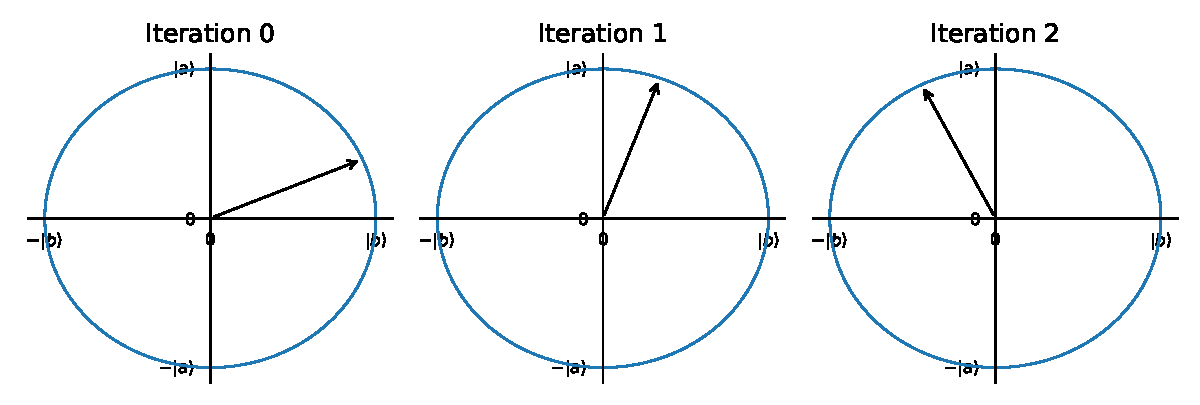
\includegraphics[width=0.85\linewidth]{graphics/q3c.pdf}
	\end{center}
    \textsf{\footnotesize{\textbf{Figure 4}: Geometric representation of Grover's algorithm iterations.}}
\end{figure}

